\subsection{Jet Trigger Efficiency}
\label{sec:jet_trigger_efficiency}

The inefficiency of the “Jet 10” trigger used to select jet events in the Run 2024 p+p dataset was investigated across the full dataset range. 

Trigger efficiencies are measured as a function of offline reconstructed jet transverse energy using minimum bias coincidence (MB) triggers as the reference. 
Unless otherwise noted, scaled trigger bits are used, which correspond to the triggered events actually collected. 
No scaledowns were applied to the "Jet 10" triggers during the Run 2024 p+p data-taking. 
The baseline efficiency definition is:
\begin{equation}
\epsilon_{\mathrm{Jet10}} =
\frac{N(\mathrm{Jet10} \cap \mathrm{MB})}{N(\mathrm{MB})}.
\end{equation}

The jet trigger efficiencies are determined using the leading uncalibrated jet transverse momentum from minimum bias and minimum bias + jet triggered events.
These uncalibrated leading jet spectra are shown for the "MB" and "Jet + MB" triggered events in Figure~\ref{fig:mb_jet_spectra}.

\begin{figure}
    \centering
    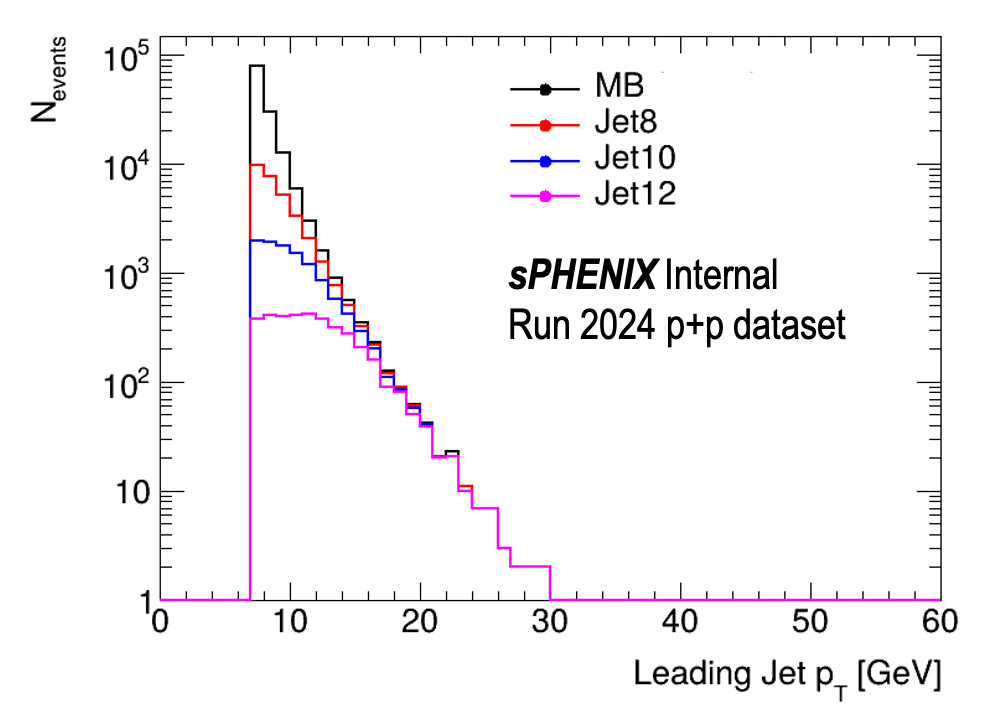
\includegraphics[width=0.7\linewidth]{ueinpp/Figures/trigger_efficiency/0mrad_all_jet_events.png}
    \caption{Comparison of the number of "MB" (black) and "MB + Jet" trigger events as a function of reconstruction-level leading jet $p_{T}$ for Jet8 (red), Jet10 (blue) and Jet12 (magenta).}
    \label{fig:mb_jet_spectra}
\end{figure}

\subsubsection{Run-by-Run Stability}

Run-by-run differences in the efficiency arise from changes in the calorimeter response and calibration across the full run dataset with consistent values for the hardware trigger conditions.
Therefore, an investigation into the statistical power of different running ranges was undertaken and implemented into the final efficiencies for the analysis.

For the majority of the Run 2024 p+p dataset, the trigger efficiency calculation is statistically limited by the amount of MB reference trigger events.
Therefore, the total number of MB reference trigger events is plotted across the full Run 2024 p+p dataset in Figure~\ref{fig:runbyrun_50pct}.
Here, there is a noticeable difference in the number of MB reference events available for use in the trigger efficiency calculation across the full run range. 

To account for these effects, the dataset is divided into three efficiency regimes all with similar statistical power: early 0~mrad, mid-time 0~mrad, and 1.5~mrad running. 
The dataset is split across time periods were runs had similar numbers of MB reference trigger events allowing for a more unbiased efficiency extraction from the run range, where no run region with particular run conditions dominates the efficiency calculation. 
This approach minimizes biases from changing calibrations and varying trigger statistics.
The resulting run range dependent efficiencies are shown in Figure~\ref{fig:jet10_vs_time_efficiency_comparison}.

\begin{figure}
    \centering
    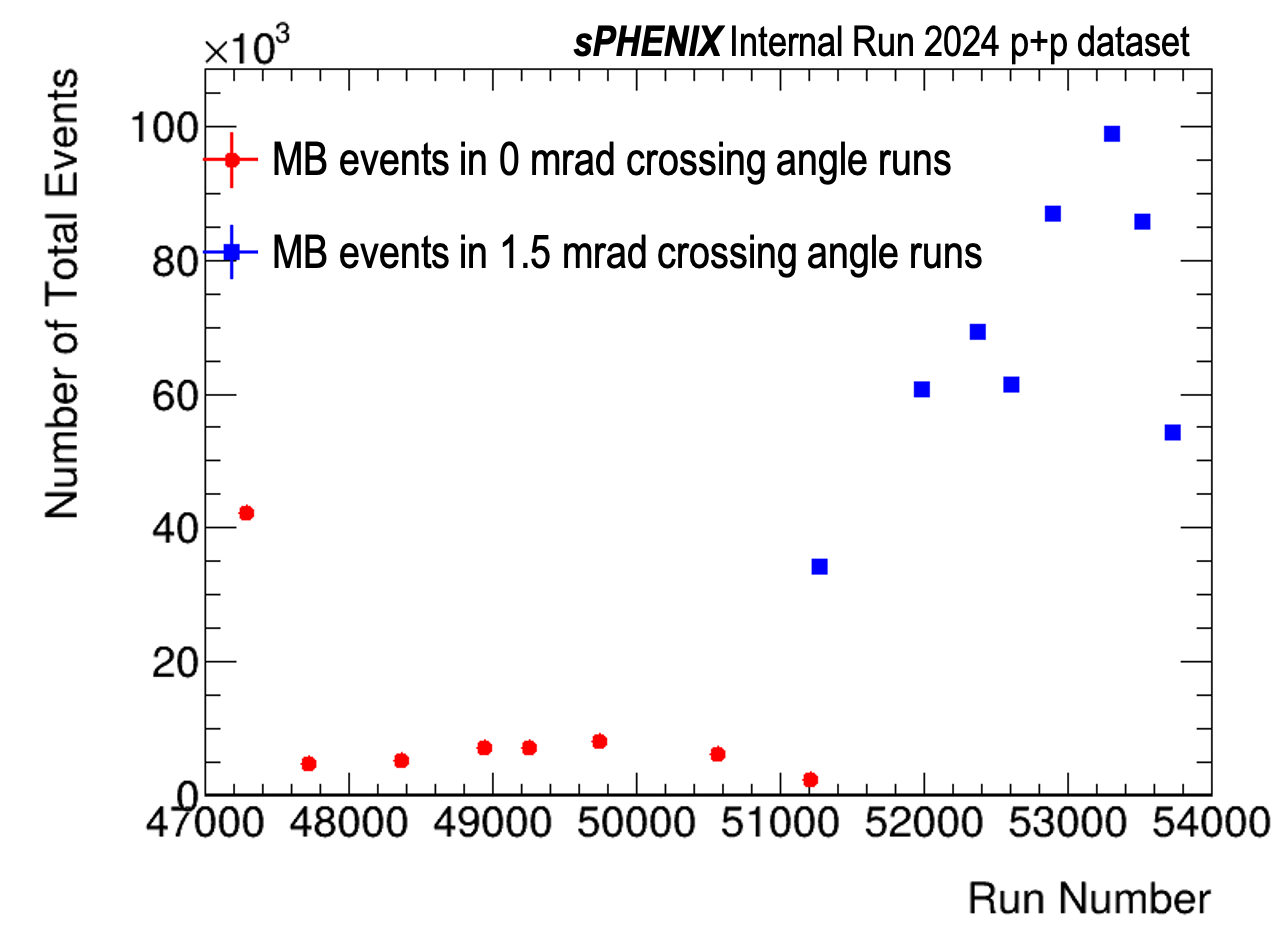
\includegraphics[width=0.7\linewidth]{ueinpp/Figures/trigger_efficiency/total_events_vs_run.png}
    \caption{Run-by-run results of total MB events with a reconstructed jet with $p_T > 7$ GeV (right).}
    \label{fig:runbyrun_50pct}
\end{figure}

\begin{figure}
    \centering
    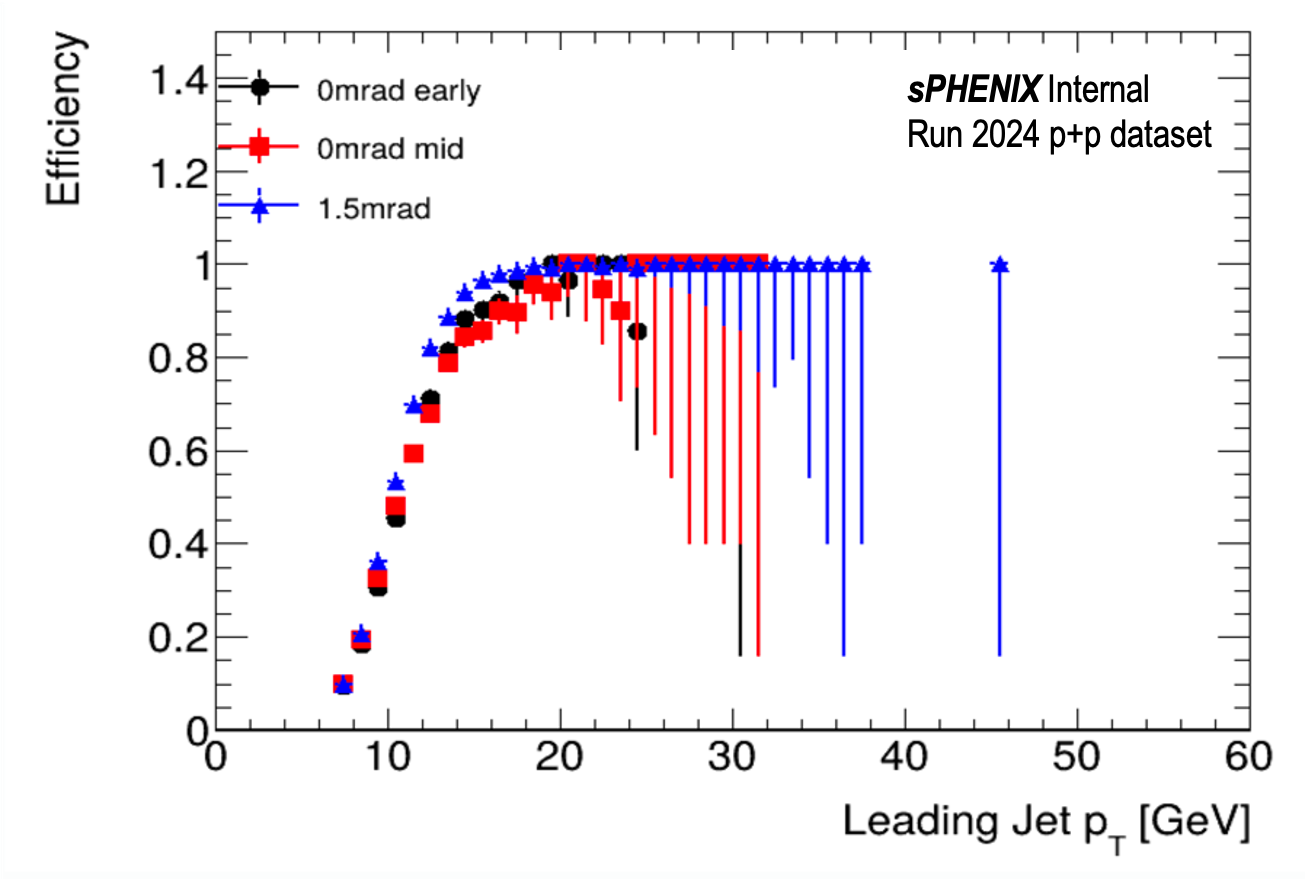
\includegraphics[width=0.7\linewidth]{ueinpp/Figures/trigger_efficiency/jet10_vs_time_efficiency_comparison.png}
    \caption{Jet10 trigger efficiency for three run ranges in the analysis: early 0 mrad (black), mid-time 0 mrad (red) and 1.5 mrad (blue).}
    \label{fig:jet10_vs_time_efficiency_comparison}
\end{figure}

\subsection{Jet Trigger Efficiency Fitting and Systematics}
\label{sec:jet_trigger_eff}

Jet trigger efficiencies are parameterized using the functional form:
\begin{equation}
    \epsilon(p_T) = [0] + [1]/pow(1+exp(-[3]*(p_T-[2])),[4])
\end{equation}
approximating a logistic turn-on behavior with asymptotic behavior at 1 (full efficiency).

Fits are performed using a binomial likelihood. 
Figure~\ref{fig:jet_trig_fitting} shows the resulting efficiency curves as a function of uncalibrated leading jet $p_{T}$. 
Statistical uncertainties are estimated by sampling the fit parameters within their covariance matrix to extract 1$\sigma$ variations. 
The overall correction from the jet trigger efficiency for the analysis range on the leading jet spectra is $< 3\%$ at 21 GeV, the start of the measurement range, and $<1\%$ for all leading jet $p_{T}$ values greater than 24 GeV.

\begin{figure}
    \centering
    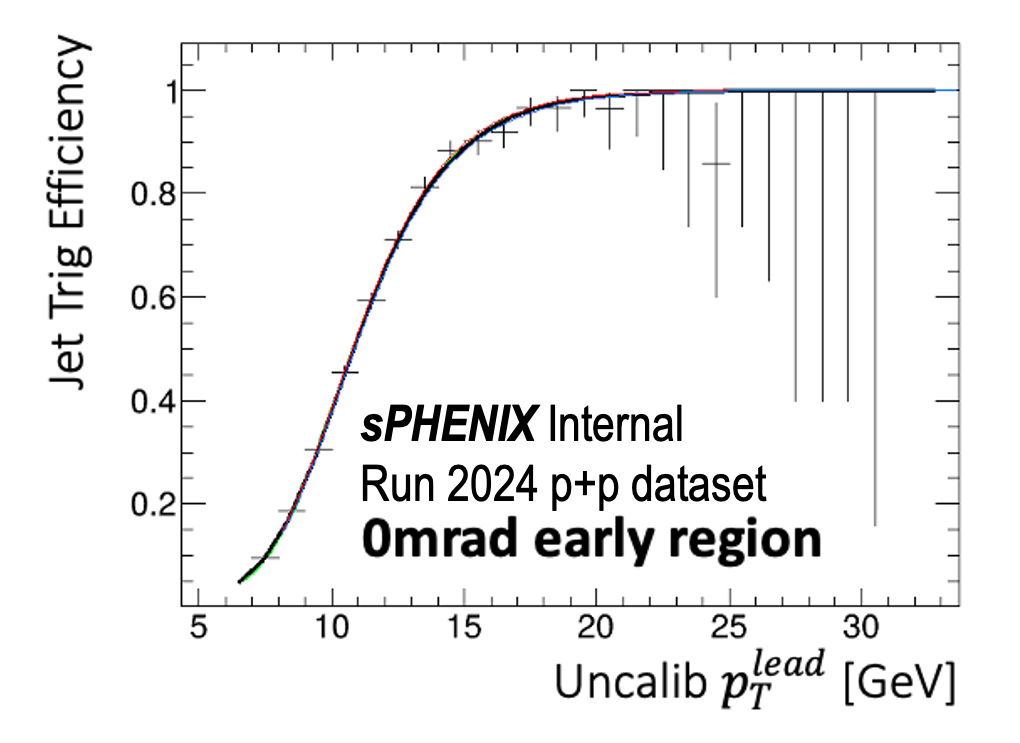
\includegraphics[width=0.48\linewidth]{ueinpp/Figures/trigger_efficiency/jet_trig_eff_fit_0mrad_early.png}
    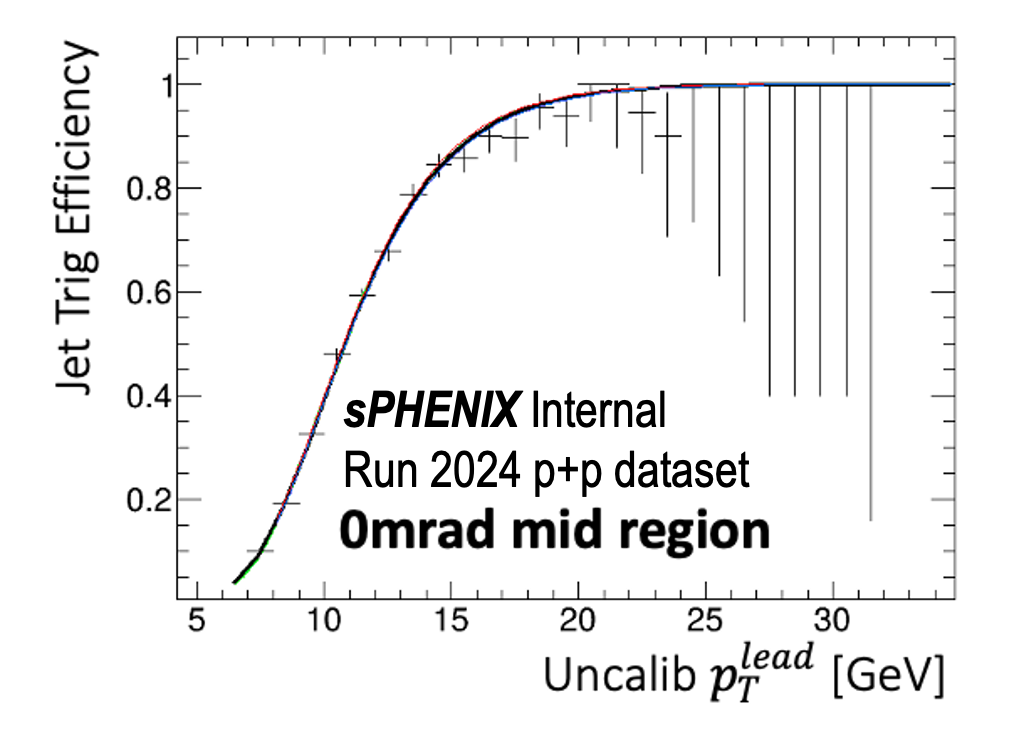
\includegraphics[width=0.48\linewidth]{ueinpp/Figures/trigger_efficiency/jet_trig_eff_fit_0mrad_mid.png}
    
\includegraphics[width=0.48\linewidth]{{ueinpp/Figures/trigger_efficiency/jet_trig_eff_fit_1.5mrad}.png}
    \caption{Jet trigger efficiency fits using data from early 0mrad (top left), mid-time 0mrad (top right) and 1.5mrad (bottom) run ranges. Nominal fit shown in black with fits defined from 1$\sigma$ variations on fit parameters shown in red/blue.}
    \label{fig:jet_trig_fitting}
\end{figure}

\subsection{MBD Vertex Efficiencies}
\label{sec:mbd_vertex_eff}

Since this analysis selects for only events with a reconstructed MBD vertex, a study of the inefficiency caused by this selection is investigated.
For this analysis, the MBD vertex efficiency determines the inefficiency at reconstructing a vertex using the MBD for a jet event with a particular jet $p_{T}$ and transverse region $E_{T}$.
Here, the vertex efficiency is evaluated in simulation and a simulation to data comparison is taken as a systematic on the simulation-based efficiency. 
Figure~\ref{fig:mbd_eff_meas_range} shows the MBD vertex efficiency both as a function of jet $p_{T}$ and transverse region $E_{T}$.

\begin{figure}
    \centering
    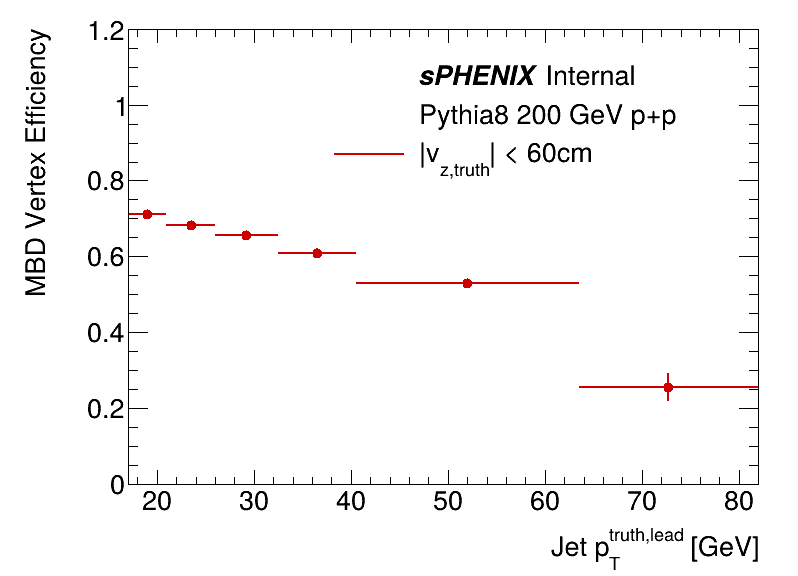
\includegraphics[width=0.48\linewidth]{figures/chapter5/mbd_vertex_eff_jet_pt.png}
    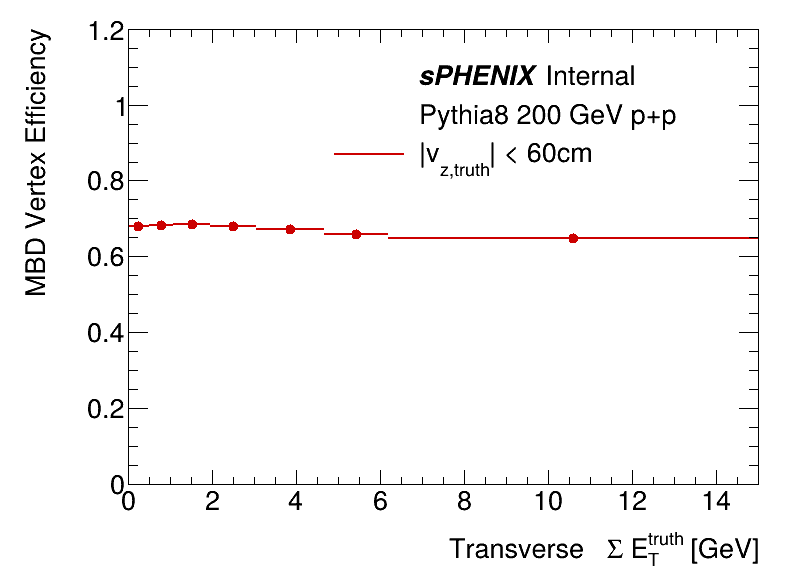
\includegraphics[width=0.48\linewidth]{figures/chapter5/mbd_vertex_eff_trans_et.png}
    \caption{MBD vertex efficiency in \pythia simulation as a function of leading jet $p_{T}$ (left) and transverse region $\Sigma E_{T}$ (right).}
    \label{fig:mbd_eff_meas_range}
\end{figure}

The transverse region dependence of the vertex efficiency is shown in Fig.~\ref{fig:mbd_eff_tr}. 
After normalizing out the dominant jet $p_{T}$ dependence, residual variations with transverse region $E_{T}$ are below the 5\% level. 
The vertex efficiency is applied at the truth level after the unfolding procedure and details on this application are provided in Section~\ref{sec:ueinpp_analysis}.

\begin{figure}
    \centering
    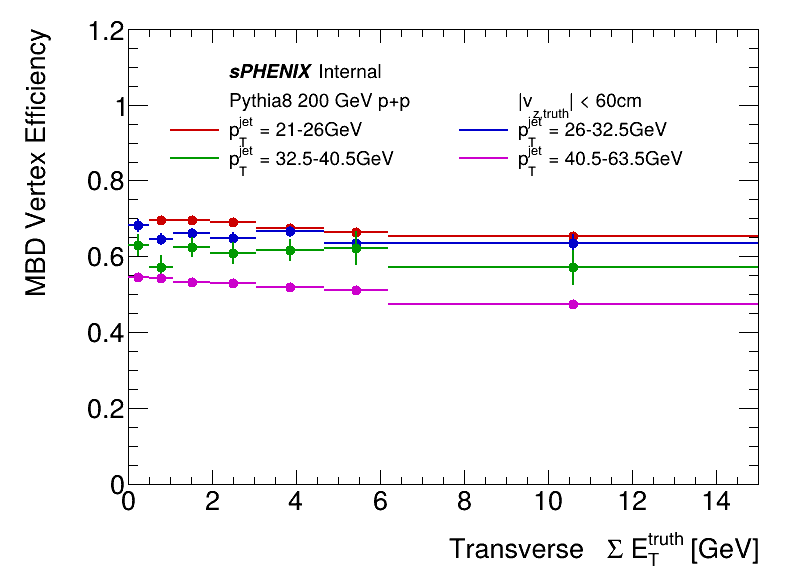
\includegraphics[width=0.48\linewidth]{figures/chapter5/mbd_vertex_eff_trans_et_jet_bins.png}
    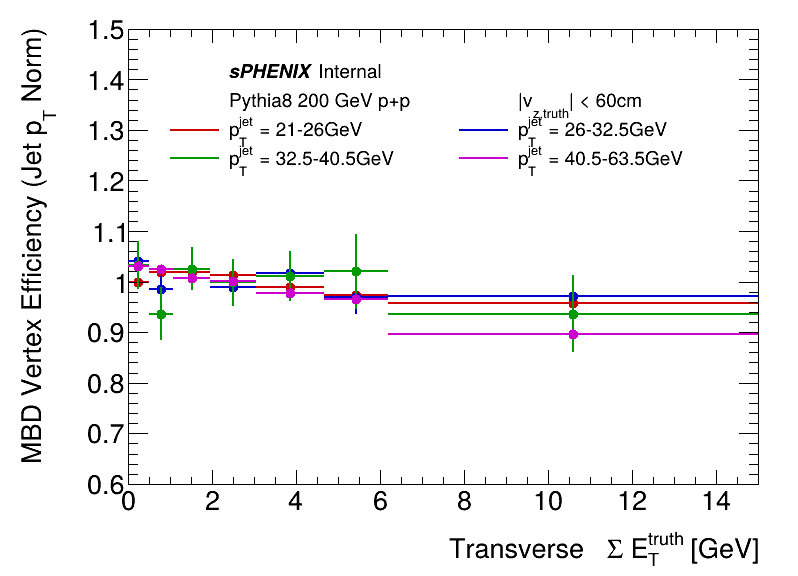
\includegraphics[width=0.48\linewidth]{figures/chapter5/mbd_vertex_eff_trans_et_jet_norm.png}
    \caption{MBD vertex efficiency in \pythia simulation as a function of transverse region $\Sigma E_{T}$ shown for slices in leading jet $p_{T}$ (left) and normalized to remove the jet $p_{T}$ dependence (right). }
    \label{fig:mbd_eff_tr}
\end{figure}

\subsection{Application of MBD Vertex Efficiency Correction}
\label{sec:mbd_vertex_eff_app}
The MBD vertex efficiency correction is applied as a scale factor to the unfolded $\Sigma E_{T}$ spectra to correct for the $\sim 5\%$ bias on the $\Sigma E_{T}$ spectra from the MBD-based vertex selection first shown in~\ref{fig:mbd_eff_meas_range}.
Figure~\ref{fig:mbd_vertex_eff_app} shows the effect of applying this efficiency correction on the unfolded $\Sigma E_{T}$ spectra and unfolding average $\Sigma E_{T}$ as a function of leading jet $p_{T}$ for both inclusive jet and dijet events. 
There is a $1\%$ effect on the average $\Sigma E_{T}$ as a function of leading jet $p_{T}$, but a nearly uniform (within 5\%) increase in the unfolded $\Sigma E_{T}$ spectra by approximately 1.4x for all $\Sigma E_{T}$ bins.

\begin{figure}
    \centering
    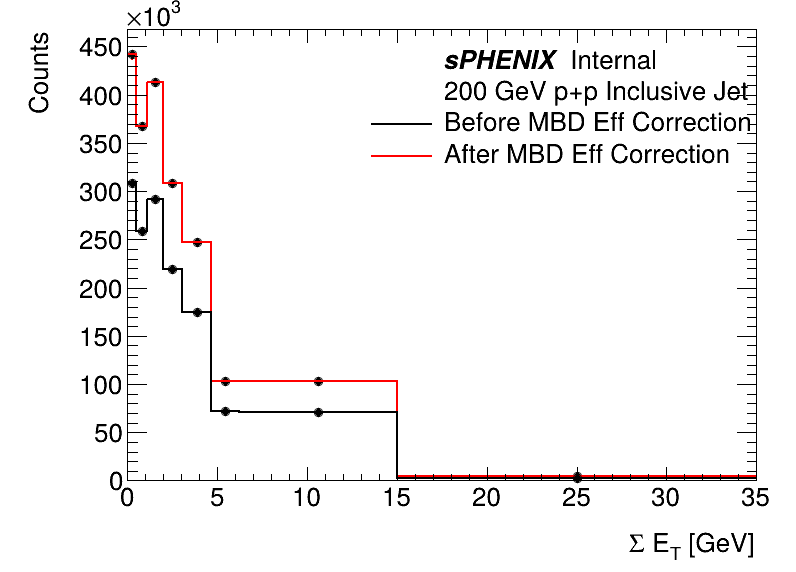
\includegraphics[width=0.48\linewidth]{ueinpp/Figures/mbd_vertex_efficiency/sphenix_primary_mbd_efficiency_effects_efrac_bkg_cut_projectionY.png}
    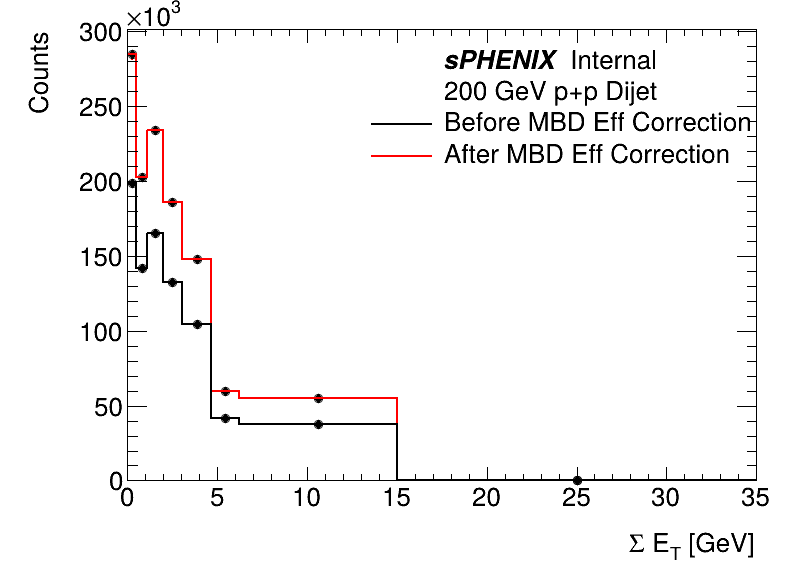
\includegraphics[width=0.48\linewidth]{ueinpp/Figures/mbd_vertex_efficiency/sphenix_primary_mbd_efficiency_effects_dijet_bkg_cut_projectionY.png}
    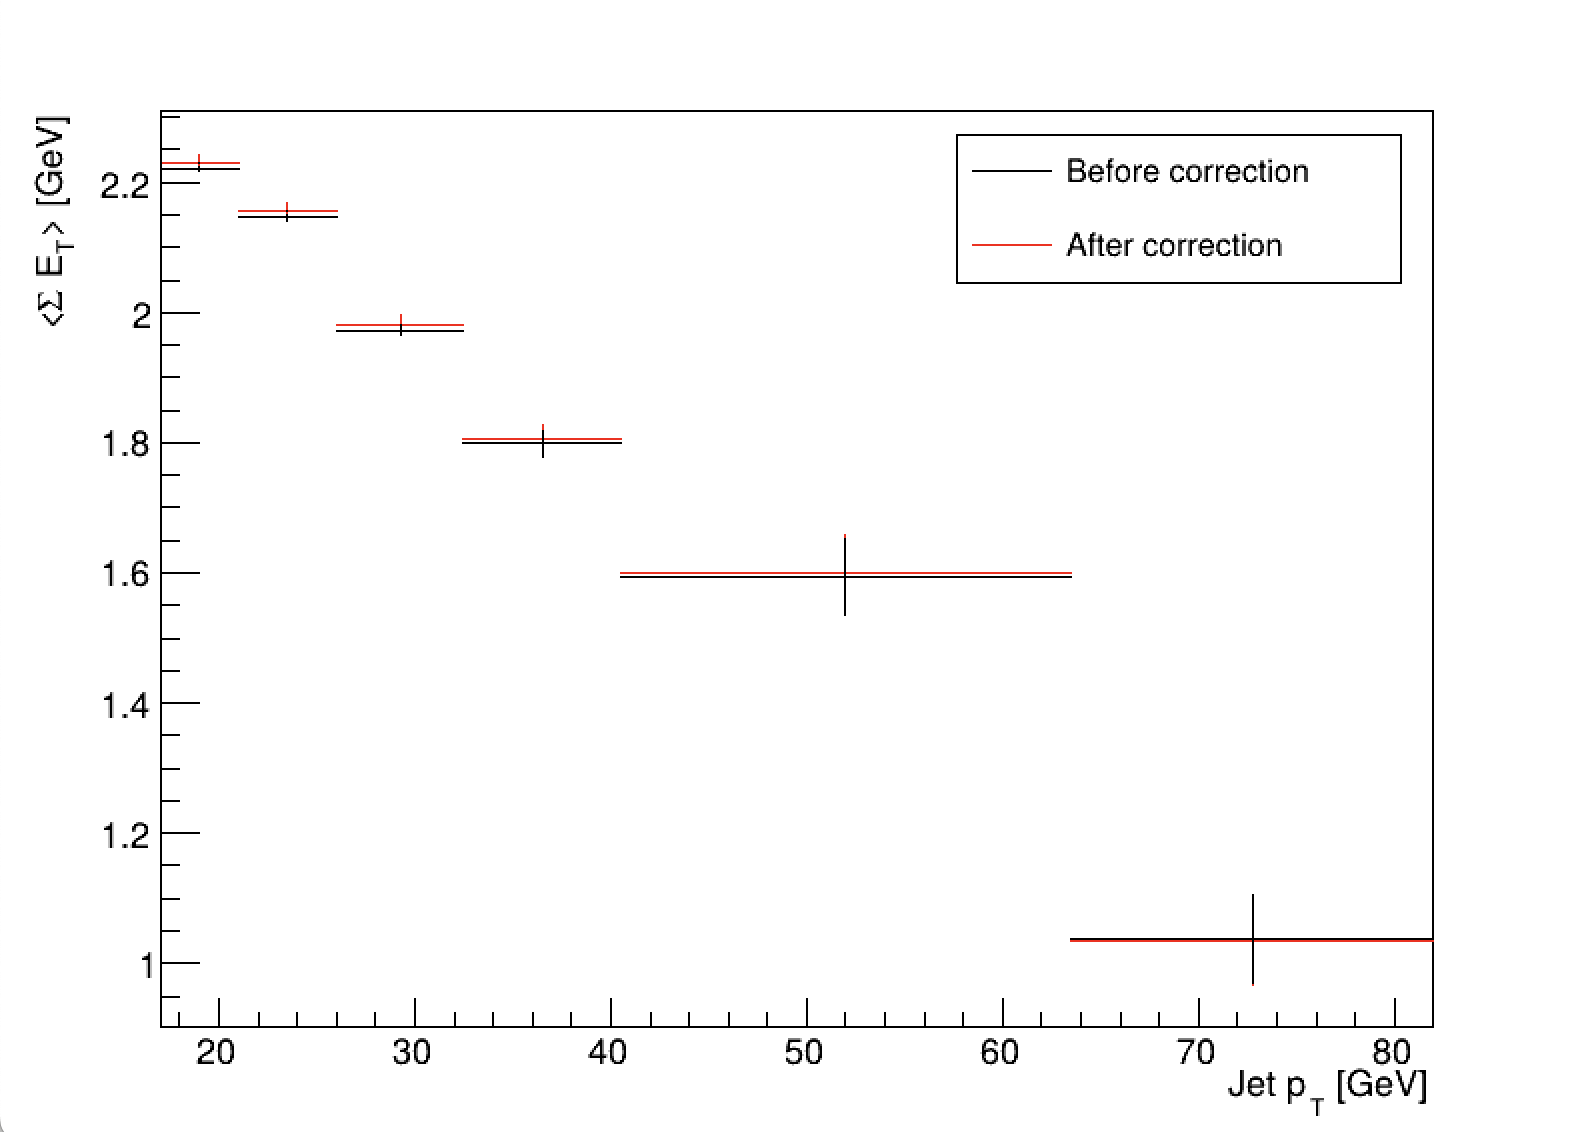
\includegraphics[width=0.48\linewidth]{ueinpp/Figures/mbd_vertex_efficiency/sphenix_primary_mbd_efficiency_effects_efrac_bkg_cut_profileX.png}
    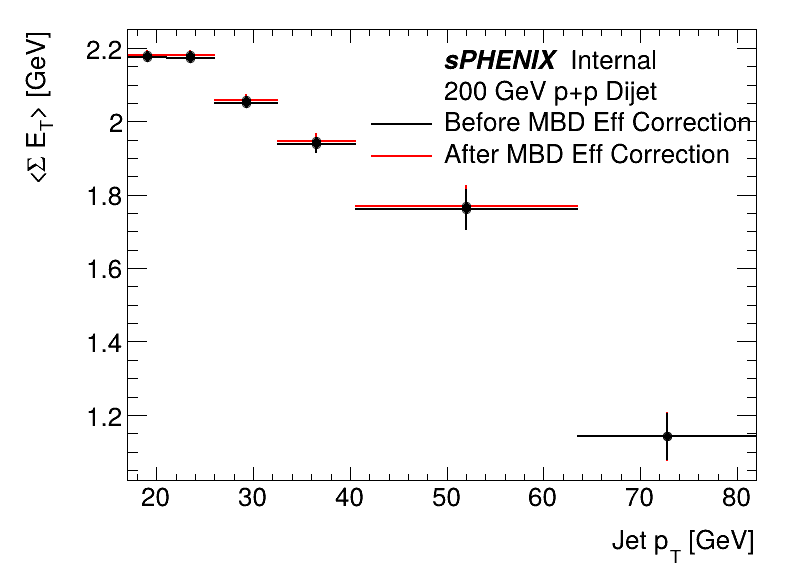
\includegraphics[width=0.48\linewidth]{ueinpp/Figures/mbd_vertex_efficiency/sphenix_primary_mbd_efficiency_effects_dijet_bkg_cut_profileX.png}
    \caption{Effect of applying MBD vertex efficiency correction on unfolded $\Sigma E_{T}$ spectra (top) and average $\Sigma E_{T}$ as a function of leading jet $p_{T}$ (bottom) for inclusive jet (left) and dijet (right) events.}
    \label{fig:mbd_vertex_eff_app}
\end{figure}
